\section{The characteristic curve for a centrifugal pump}



\subsection{Theoretical head}

The theoretical head corresponds to the total energy conveyed by the
rotor to the fluid, and follows from Euler's equation:
\begin{align*}
  \dhead_i = \frac{\fVel_2 \aVel_{u2} - \fVel_1 \aVel_{u1}}{\grav}
\end{align*}

At both the in- and outlet station, the radial velocity can be
computed from the impeller flow rate
\begin{align*}
  \rVel_{r1} &= \aVel_{r1} = \frac{\vFlow_i}{2 \pi  R_1 b_1 k_1} \\
  \rVel_{r2} &= \aVel_{r2} = \frac{\vFlow_i}{2 \pi  R_2 b_2 k_2} \\
\end{align*}
where $b_1$ and $b_2$ are the channel heights and $k_1$ and $k_2$
blockage factors due to the presence of the blades.  At the inlet, the
absolute flow angle $\alpha_1$ is supposedly known.  Therefore we have
\begin{align*}
  \aVel_{u1} &= \aVel_{r1} \tan \alpha_1
  \rVel_{u1} &= \aVel_{u1} - \fVel_{u1} = \aVel_{u1} - \rot R_1
\end{align*}
In case the impeller has an infinite number of blades, the relative
velocity follows the blade perfectly; at the outlet, the relative flow
angle $\beta_2$ then corresponds to the blade outlet metal angle.
\begin{align*}
  \rVel_{u2} &= \rVel_{r2} \tan \beta_2 \\
  \aVel_{u2} &= \rVel_{u2} + \fVel_2 = \rVel_{u2} + \rot R_2
\end{align*}
The head is thus
\begin{equation}
  \dhead_{i\infty} = \frac{\rot^2 R_2^2}{\grav} + 
  \frac{\rot}{2 \pi \grav} \left(
    \frac{\tan \beta_2}{k_2 b_2} - 
    \frac{\tan \alpha_1}{k_1 b_1}\right) \vFlow_i
\end{equation}
In case no pre-rotation is present (\ie $\alpha_1=0$), we find that
the blade outlet angle determines the slope of the characteristic
curve $\dhead_{i\infty} = \dhead_{i\infty}(\vFlow_i)$: 
\begin{itemize}
\item for a backward bent blade (a), an increase of the velocity
  decreases $\aVel_{u2}$ and therefore the work. This configuration is
  desirable since it provides a moderate blade loading in the
  impeller, and therefore a better evolution of the performance away
  from the design point, as well as a stable operating curve, as will
  be discussed later on.
\item for a purely radial blade (b), the outlet tangential velocity is
  not changed by the flow rate since $\aVel_{u2} = \fVel_2$ and
  therefore the head rise is theoretically independent of flow rate;
  however losses will significantly alter the real head curve.
\item for a forward bent blade (c), an increase of the flow rate
  increases $\aVel_{u2}$ and therefore the head. The impeller is
  characterized by very high loading since the flow undergoes a very
  drastic change of direction, from $\beta_1 < 0$ to $\beta_2 >
  0$. The (absolute) exit velocity is very high and therefore a very
  important part of the static head rise needs to be obtained in the
  diffuser. Another issue is the unstable nature of the head curve, as
  will be discussed later on.
\end{itemize}

\begin{figure}[!h]
  
  \begin{subfigure}{\textwidth}
    \centering{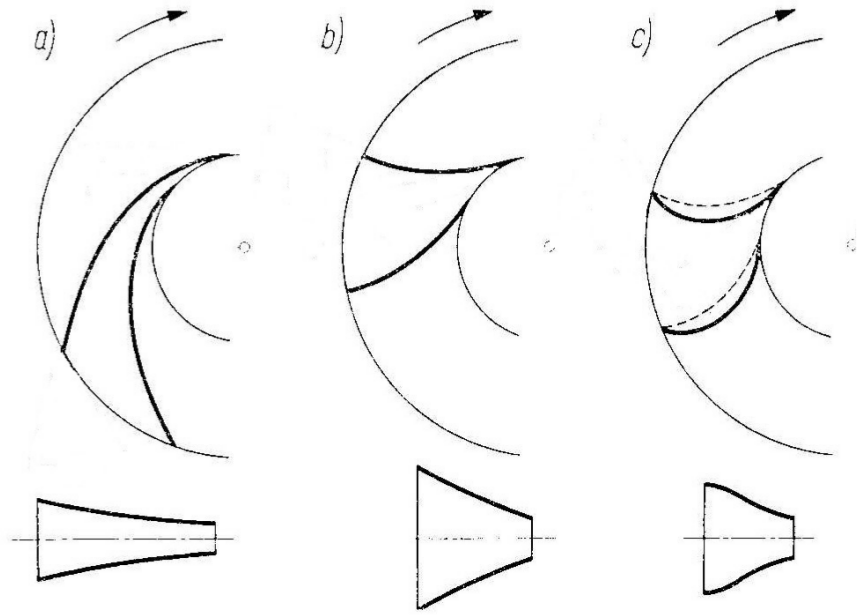
\includegraphics[width=0.6\textwidth]{pumps/characteristicSlope.png}}
    \caption{Blade geometry}
  \end{subfigure}
  \vspace{2ex}
  \begin{subfigure}{\textwidth}
    \centering{
      \includegraphics[width=0.8\textwidth]{pumps/characteristicSlope2.tikz}}
      \caption{Modification of the velocity triangle for $\textcolor{red}{\vFlow^\prime} > \vFlow_n$}
  \end{subfigure}

  \vspace{2ex}
  \begin{subfigure}{\textwidth}
    \centering{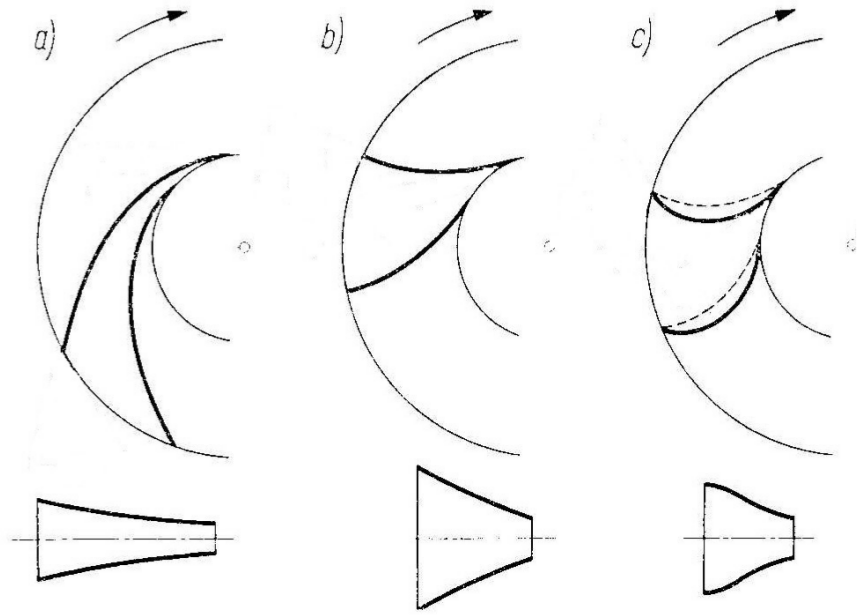
\includegraphics[width=0.6\textwidth]{pumps/characteristicSlope.tikz}}
    \caption{Theoretical head evolution}
  \end{subfigure}
  
  \caption{Impact of outlet angle on characteristic curve. (Backward/radial/forward blades).}
  \label{fig:slopeCharacteristic}
\end{figure}


\subsection{Slip factor}



\subsection{Losses}


The theoretical head is the head which would be generated for the same
power, if no losses were incurred. In reality, it supports the pump
head $\dhead_p$ and the hydraulic losses $\loss_{oi}$ in the pump. The
loss mechanisms were previously discussed in chapter
\ref{sec:pumps:hydrodynamicLosses}.

\subsubsection{Distributor losses}

The losses in the distributor are mainly due to friction, and modeled
as:
\begin{align*}
  \loss_{d1} = k_{d1}\frac{\vel_1^2}{2g}
\end{align*}

\subsubsection{Impeller losses}

The first losses concern incidence losses at impeller inlet,
associated to the misalignment of the flow with the blades at
off-design conditions. The velocity triangle entering the impeller
(station $1$)can be deduced from the velocity leaving the inlet guide
vanes (station $1^\prime$).
\begin{itemize}
\item the throughflow velocity $\aVel_m$ should be corrected for the
  throughflow surface, due to changes in radius $R$, passage height
  $b$ and blockage $k$ in the impeller blades 
  \begin{align*}
    \aVel_{m1} = \frac{R_{1^\prime} b_{1^\prime} k_{1^\prime}}{R_1 b_1 k_1} \aVel_{m1^\prime}
  \end{align*}
\item due to conservation of moment of momentum we have 
  \begin{align*}
    \aVel_{u1} = \frac{R_{1^\prime}}{R_1} \aVel_{u1^\prime}
  \end{align*}
\end{itemize}
As demonstrated before, these losses are of the form:
\begin{align*}
  \loss_{11^\prime} = k_1 \frac{\fVel^2_1}{2\grav} 
  \left(\frac{\vFlow_n-\vFlow}{\vFlow_n}\right)^2
\end{align*}
Since the factors involved in the change in the absolute velocity from
station $1^\prime$ to $1$ are purely geometrical, they can be taken up
in the factor $k_1$.  

The second source of losses concern friction losses in the impeller
channel. These losses will be locally proportional to
$\rVel^2$. Therefore, we choose a representative velocity to compute
the friction loss, \eg at outlet, such that
\begin{align*}
  \loss_{12} = k_{12} \frac{\rVel_2^2}{2 \grav}
\end{align*}

\subsubsection{Diffuser losses}

When leaving the impeller at station 2 and entering the diffuser at
station $2^\prime$, we will again have the same type of modifications
of the absolute velocity as before:
\begin{align*}
  \aVel_{m2^\prime} = \frac{R_{2} b_{2} k_{2}}{R_2^\prime b_2^\prime k_2^\prime} 
  \aVel_{m2}
  \aVel_{u2^\prime} = \frac{R_{2}}{R_2^\prime} \aVel_{u2}
\end{align*}
And then again the incidence losses are computed as 
\begin{align*}
  \loss_{22^\prime} = k_2 \frac{\fVel^2_2}{2\grav} 
  \left(\frac{\vFlow_n-\vFlow}{\vFlow_n}\right)^2
\end{align*}
since the factors involved in the change in the absolute velocity are
purely geometrical, they can be taken up in a correction factor $k_2$.  

\subsubsection{Volute entrance losses}

In case no diffuser is present, dump diffusion is used for two reasons:
\begin{itemize}
\item realise a first rapid recuperation of kinetic energy from the
  throughflow component;
\item ensure a more tangential flow in order to arrive at a more
  compact volute.
\end{itemize}
The head loss associated to the 


\def\Q{10}
\def\Qn{3}
\def\Qm{9}
\def\Hm{4}
\begin{figure}[!h]
  \centering{
\def\Q{10}
\def\Qn{3}
\def\Qm{9}
\def\Hm{4}
\def\fCoef{0.2}
    
\tikzsetnextfilename{characteristic}
\begin{tikzpicture}

  \coordinate(origin) at (0,0);
  \coordinate(maxQ) at (\Qm,0);
  \coordinate(maxH) at (0,\Hm);
  \coordinate(maxX) at (\Qm*1.2,0);
  \coordinate(maxY) at (0,\Hm*1.2);

	%\coordinate(p11) at ((\Qm*(1-sqrt(1-4*(1-\fCoef)*\fCoef*\fCoef))/2/\fCoef),0);								 
	%\draw node(lala) at (p11)[below]{$\vFlow_{max}$};
				
  \begin{axis}[
	  width = 0.8\textwidth,
		height =0.3\textheight,
	  xtick = \empty,
		ytick = \empty,
		axis lines = center,
		xmin = 0,
		ymin = 0,
		xmax = 1.2*\Qm,
		ymax = 1.2*\Hm,
		xlabel = $\vFlow$,
		ylabel = $\head$],
		\addplot [domain=0:\Qm,blue]{\Hm*(1-x/\Qm)} node[pos=\Qm]{$\head_i$};
		\addplot [domain=0:1.1*\Qm,red]{\Hm*\fCoef*(x/\Qm)*(x/\Qm)} node[pos=\Qm]{$\loss_f$};
		\addplot [domain=0:\Qm]{\Hm*((1-x/\Qm)-\fCoef*(x/\Qm)*(x/\Qm))} node[pos=\Qm]{$\head_i - \loss_f$};
	\end{axis}		 
\end{tikzpicture}
}
\end{figure}


%%% Local Variables: 
%%% mode: latex
%%% TeX-master: "../MECA0467"
%%% End: 
